\documentclass{standalone}
\usepackage{pgfplots}
\pgfplotsset{compat=newest}

\begin{document}
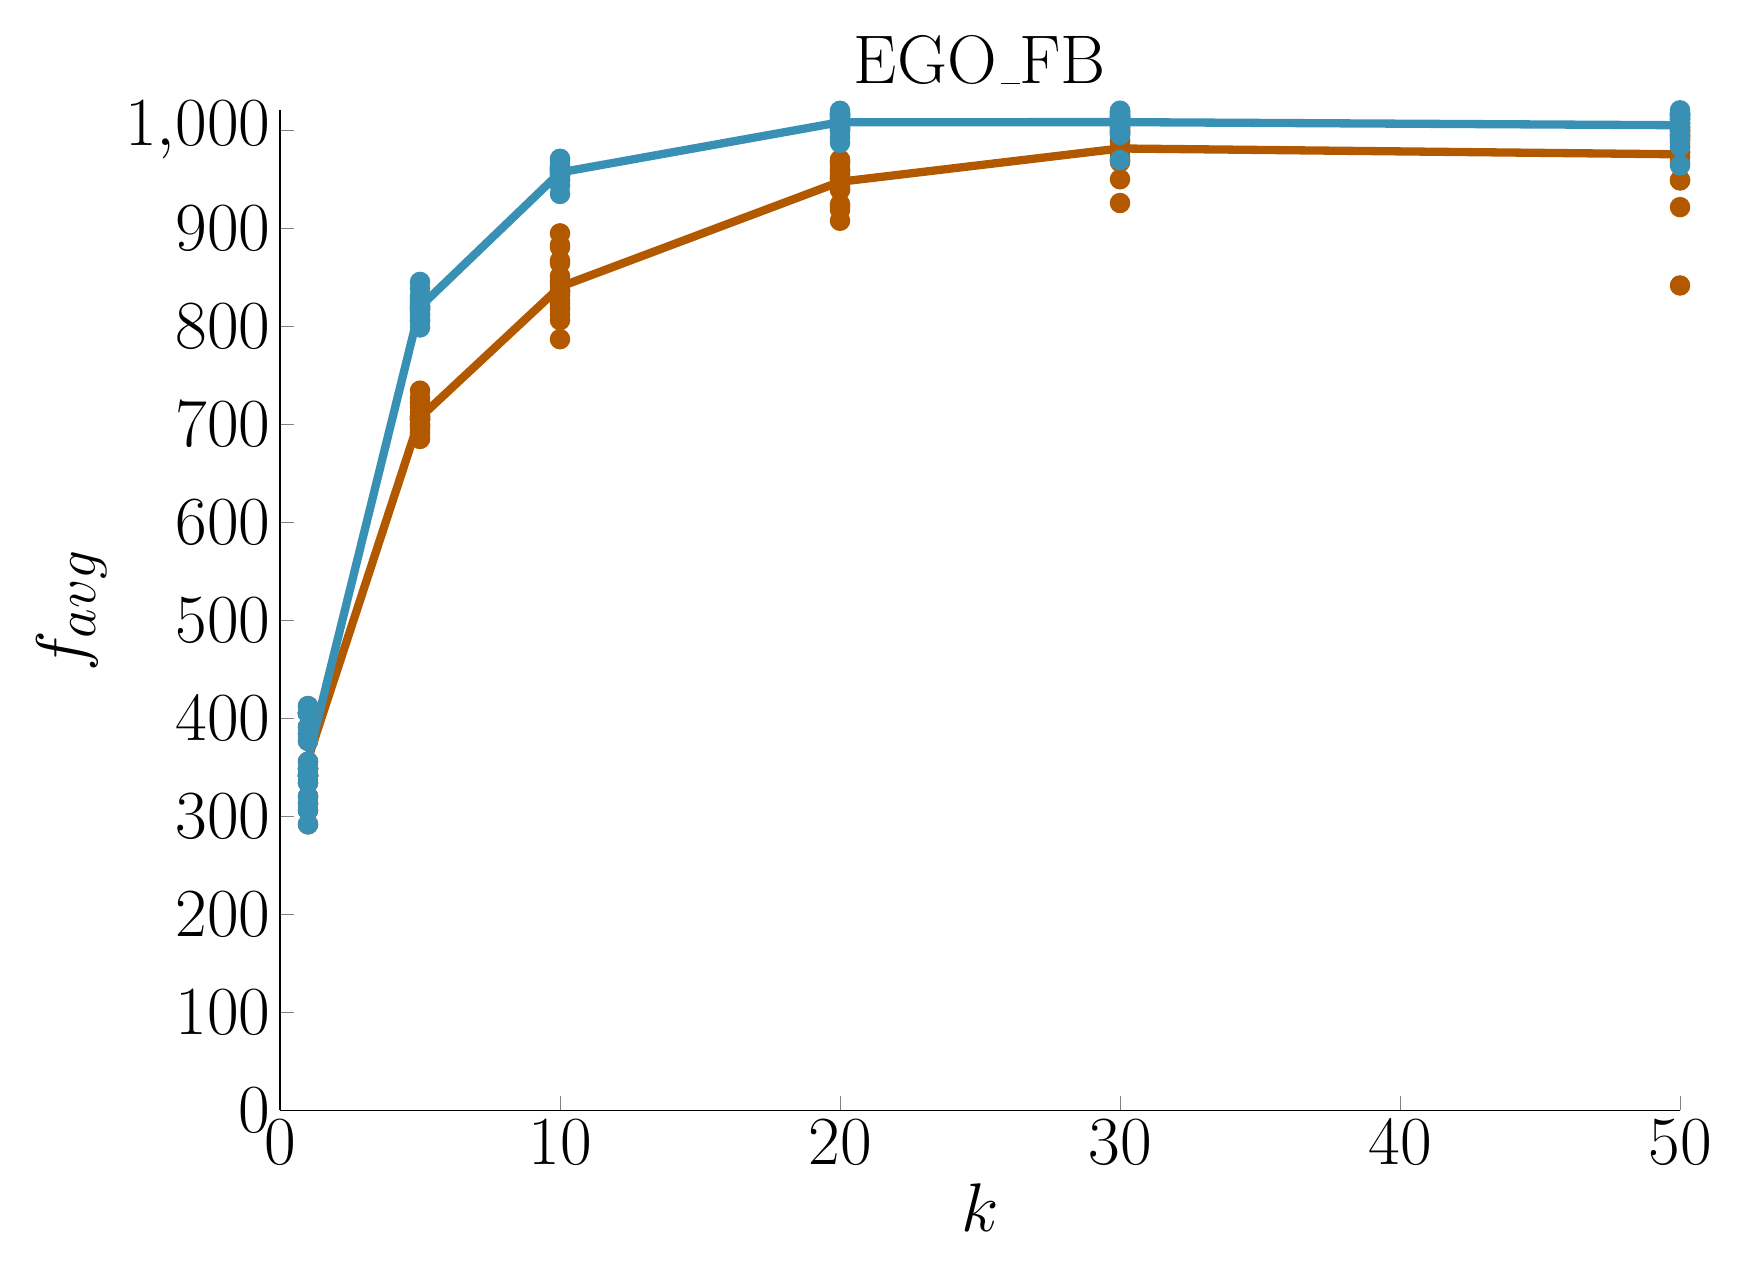
\begin{tikzpicture}

\begin{axis}[%
title style={font=\Huge},
title=EGO\_FB,
tick label style={font=\Huge},
label style={font=\Huge},
legend style={font=\Huge},
view={0}{90},
max space between ticks=50pt,
width=7in,
height=5in,
scale only axis,
xmin=0, xmax=50,
xtick={0, 10, 20, 30, 40, 50},
xlabel={$k$},
ymin=0, ymax=1019.89,
%ytick={0, 200, 400, 600, 800, 1000},
ylabel={$f_{avg}$},
major tick length=5pt,
axis lines*=left,
legend cell align=left,
clip=false]

\addplot [
only marks,
mark=*,
mark size=3.5pt,
color=orange!70!black,
%solid,
%line width=2pt,
]
coordinates{
(1,291.69)(1,305.87)(1,312.96)(1,320.05)(1,334.23)(1,341.32)(1,341.32)(1,341.32)(1,341.32)(1,348.41)(1,348.41)(1,355.5)(1,376.77)(1,383.86)(1,390.95)(1,405.13)(1,405.13)(1,405.13)(1,405.13)(1,412.22)(5,684.7)(5,689.39)(5,691.38)(5,695.3)(5,697.08)(5,698.41)(5,699.82)(5,704.13)(5,704.19)(5,704.48)(5,705.8)(5,706.71)(5,707.28)(5,708.47)(5,712.15)(5,717.36)(5,721.45)(5,722.86)(5,726.33)(5,733.93)(10,786.46)(10,805.85)(10,811.91)(10,816.81)(10,818.85)(10,822.7)(10,826.4)(10,831.7)(10,834.89)(10,835.33)(10,836.26)(10,841.05)(10,844.19)(10,846.05)(10,850.81)(10,864.01)(10,866.61)(10,880.37)(10,882.4)(10,894.38)(20,907.24)(20,918.46)(20,921.7)(20,924.09)(20,938.64)(20,939.46)(20,940.97)(20,945.04)(20,949.76)(20,950.1)(20,951.41)(20,952.5)(20,955.3)(20,957.73)(20,958.55)(20,959.95)(20,965.36)(20,966.27)(20,968.27)(20,969.49)(30,925.31)(30,949.57)(30,967.14)(30,969.01)(30,972.18)(30,977.24)(30,977.95)(30,978.54)(30,980.99)(30,981.2)(30,981.25)(30,983.77)(30,988.02)(30,989.94)(30,996.81)(30,998.63)(30,998.89)(30,999.37)(30,1001.43)(30,1002.06)(50,841.24)(50,921.13)(50,948.41)(50,948.66)(50,965.85)(50,972.0)(50,976.79)(50,977.43)(50,982.06)(50,986.21)(50,990.9)(50,993.42)(50,993.7)(50,994.92)(50,998.31)(50,998.84)(50,999.6)(50,1001.22)(50,1003.02)(50,1006.47)
};

\addplot [
only marks,
mark=*,
mark size=3.5pt,
color=cyan!70!black,
%solid,
%line width=2pt,
]
coordinates{
(1,291.69)(1,305.87)(1,312.96)(1,320.05)(1,334.23)(1,341.32)(1,341.32)(1,341.32)(1,341.32)(1,348.41)(1,348.41)(1,355.5)(1,376.77)(1,383.86)(1,390.95)(1,405.13)(1,405.13)(1,405.13)(1,405.13)(1,412.22)(5,798.45)(5,804.94)(5,805.38)(5,807.74)(5,810.73)(5,812.4)(5,816.34)(5,816.54)(5,816.91)(5,818.8)(5,819.51)(5,819.6)(5,821.49)(5,823.31)(5,825.91)(5,827.07)(5,829.52)(5,830.21)(5,837.88)(5,844.87)(10,934.57)(10,943.13)(10,948.19)(10,949.03)(10,952.13)(10,953.79)(10,954.38)(10,956.49)(10,956.52)(10,956.92)(10,958.24)(10,958.98)(10,959.68)(10,960.31)(10,961.56)(10,961.94)(10,962.12)(10,963.74)(10,968.36)(10,970.48)(20,986.74)(20,991.91)(20,998.23)(20,999.49)(20,1000.58)(20,1001.82)(20,1002.91)(20,1007.47)(20,1009.7)(20,1010.13)(20,1010.37)(20,1010.49)(20,1013.32)(20,1013.53)(20,1013.68)(20,1015.95)(20,1016.19)(20,1016.21)(20,1017.12)(20,1019.35)(30,969.13)(30,994.75)(30,995.6)(30,995.64)(30,996.23)(30,1002.75)(30,1003.86)(30,1011.31)(30,1012.33)(30,1012.53)(30,1013.06)(30,1013.66)(30,1013.88)(30,1014.48)(30,1015.84)(30,1016.78)(30,1017.85)(30,1018.74)(30,1018.87)(30,1019.45)(50,963.67)(50,982.98)(50,988.81)(50,990.37)(50,994.15)(50,996.07)(50,1002.24)(50,1006.57)(50,1007.18)(50,1010.38)(50,1010.86)(50,1011.79)(50,1013.89)(50,1014.02)(50,1014.63)(50,1015.89)(50,1016.45)(50,1016.46)(50,1017.04)(50,1019.89)
};

\addplot [
color=orange!70!black,
solid,
line width=3pt
]
coordinates{
(1,358.336)(5,706.561)(10,839.8515)(20,947.0145)(30,980.965)(50,975.009)
};

\addplot [
color=cyan!70!black,
solid,
line width=3pt
]
coordinates{
(1,358.336)(5,819.38)(10,956.528)(20,1007.7595)(30,1007.837)(50,1004.667)
};


\end{axis}
\end{tikzpicture}
\end{document}
